% !TEX root = ./paper.tex
%---------------------
\section{Introduction}
%---------------------

% !TEX root = ./paper.tex
The Transmission Control Protocol (\tcp) \cite{rfc793} is one of the most
critical protocols in today's Internet. It has been designed following a
layer approach and now serves a wide range of
applications. During the last four decades, \tcp evolved under
the pressure of competing protocols. In the 1980s, software-based \tcp
implementations were considered too slow. Researchers proposed new transport
protocols such as \xtp~\cite{sanders1990xpress} which could be implemented in
hardware. Meanwhile, \tcp implementations got a considerable speed
boost~\cite{clark1989analysis} and \xtp disappeared. The \tcp speed boost and
usage triggered the development of various important \tcp extensions, including
timestamps and large windows~\cite{rfc1323} or Selective
Acknowledgments~\cite{rfc2018}.

In the mid-nineties, the Secure Socket Layer (\ssl) protocol was proposed as an
additional layer to \tcp to secure emerging e-commerce
websites~\cite{draft-hickman-netscape-ssl}. \ssl evolved in different versions
of the Transport Layer Security (\tls) protocol, the most recent one being
version 1.3~\cite{rfc8446}. %Many details of the \tls protocol have changed
%since the first version of SSL~\cite{kotzias2018coming}.
Nowadays, \tls is almost ubiquitous on web servers~\cite{holz2019era} and many
non-web applications use it~\cite{anderson2019tls}.

During the late nineties, early 2000s, transport protocol researchers explored
alternatives to \tcp. The IETF standardized two new transport protocols:
\dccp~\cite{kohler2006designing} and \sctp~\cite{rfc4960}. We rarely use \dccp
today. Despite \sctp benefits (support for multihoming, better design, and
extensibility), only niche applications use it. %This limited deployment is
%probably due to two different factors. First, \sctp forced the applications to
%%%<--(mp): c'est aussi ce qu'a fait quic et tcpls
%use a new API.
This limited deployment is mainly due to the various middleboxes (NAT,
firewalls, etc.) deployed in
the Internet often blocking packets that do not carry \tcp or
\udp~\cite{honda2011still}.  \sctp initially supported multihoming by switching
from one path to another. It was later extended to use different
paths continuously~\cite{iyengar2006concurrent}. Multipath
\tcp~\cite{rfc6824,raiciu2012hard} brought similar capabilities to \tcp, and
included a coupled congestion control scheme~\cite{wischik2011design}, later
brought to \sctp as well. This particular succession of events shows how
different designs compete and advance each other.

Extending \tcp today is not feasible anymore as middleboxes severely interfere
with changes to the \tcp header and
options~\cite{medina2004measuring,honda2011still,edeline2019bottom}.
To overcome this problem, Google started \quic as an experimental
protocol~\cite{roskind2013quic,langley2017quic} combining functions usually
found in \tcp, \tls, and HTTP/2. During the last years, it
evolved into a complete transport protocol~\cite{rfc9000}.
%whose standardization is being finalized within the IETF
\quic leverages encryption to prevent middlebox interference and propose to
revisit the layered model of the Internet to improve the transport services.
%Indeed, the integration of \tls 1.3 allows 1-RTT secure
%handshakes and extensive packet encryption, providing more security and
%preventing middlebox interference.
%A key characteristic of \quic is that it encrypts almost all the packets, including most of their
%headers.
As \quic runs atop \udp, it can be implemented and deployed as a user-space library.
%Although \quic is essentially a new transport protocol, it does not run
%directly above IP in contrast with \sctp or \tcp. \quic runs above \udp, enabling
%user-space implementation as a library and overcoming middleboxes that filter IP.
%With this choice, \quic can be implemented as a user-space library, and \quic packets
%can pass through middleboxes.

Does the standardization of \quic marks the end of the \tcp era, moving
all applications and transport research to \quic?  We do not think
so. Today, \quic is mainly used for HTTP/3~\cite{http3} and \tcp remains a
fallback because of its greater support in networks. \tcp also still serves many  applications~\cite{covid19,fiveyears}.
%In the future, TCP will remain the fallback for QUIC because of its greater
%supportin networks.
%
%History tells us that \tcp has evolved with competing transport protocols.
In the light of those recent advances, we revisit how transport services can be
provided with \tcp and \tls today. The \quic design integrates services
that were found in the security and application layers, e.g., encryption and multiplexing.
\tcp and \tls have been both designed in strict layers separating the two.
%\quic is today's competitor and but there is still plenty of room to improve \tcp.
This paper revisits this separation through the lens of the following research questions:

\begin{itemize}
	\item[{\small{\textit{RQ1}}} -] How can \tcp and \tls be
	combined to improve extensibility and middlebox resilience ?
  %\todo{Discuss middleboxes and TCP extensibility so that the
	%question can become: How can TCP and TLS be combined to alleviate middlebox
	%interference or smth.}
%  \item[{\small{\textit{RQ2}}} -] How can we alleviate middlebox
%    interferences?
	\item[{\small{\textit{RQ2}}} -] What are the new transport services this
	combination can offer?
	%\item[{\small{\textit{RQ3}}} -] How do these services compete with other
	%protocols ?
\end{itemize}

To answer these questions, we design and implement an approach that combines
\tcp and \tls 1.3 into a fast, flexible, and secure transport protocol called \textbf{\tcpls}.
%
%In this paper, we take a step back. As \quic closely couples the reliability and
%security mechanisms, we reconsider the separation between \tcp and \tls.  In
%this paper, we combine both \tcp and \tls 1.3 in a single fast, flexible, and
%secure protocol called \textbf{\tcpls}
\footnote{A preliminary version of this work has been presentend in a workshop
  paper~\cite{rochet2020tcpls}.}  At the heart of our approach, we illustrate
how \tls records (i.e., messages exchanged through \tls) can be leveraged to
build new transport services. In \tcp/\tls, \tls \texttt{AppData} records are
solely used to securely convey the \tcp bytestream. In \tcpls, we extend their
use to convey both application and control data including encrypted \tcp
options.
%\todo{more detail needed?}

We demonstrate that this combination allows secure extensibility that can also
be used with techniques such as \tcp Fast Open \cite{rfc7413} to lower the
handshake latency. We leverage this new extensibility to implement modern transport services such as multiplexing, connection migration, and stream steering capabilities without risking middlebox interference. Our \tcpls prototype is implemented as a user-space library exposing a powerful API to applications % around a Stream %Steering mechanic
while leveraging the high-performance Linux kernel \tcp stack. Our lab measurements indicate that \tcpls can be implemented at a low cost while providing more bulk throughput and features than the \quic implementations we tested.
%(mp): Je n'aime pas trop cette notion de flexibilité que l'on ne définit jamais vraiment

%We have
%designed \tcpls with three goals in mind. First, \tcpls exposes modern transport
%features, such as multipath capabilities, to the application. Second, \tcpls
%solves \tcp's extensibility issues in \tcp by relying on the \tls handshake for
%\tcp options negotiation and by including \tcp options inside \tls records.
%Finally, we draw a path to make \tcpls an excellent challenger to \quic.  With that in mind, we have implemented \tcpls as a user-space library that exposes a powerful API to applications but still relies on the high-performance in-kernel \tcp stack. Our implementation uses \tls' flexible record layer to create a secure control channel that the \tcpls session endpoints can use to exchange
%control information. This channel enables different use cases such as connection
%migration or seamless failovers without risking middlebox interference.

%Our lab
%measurements indicate that our \tcpls prototype outperforms existing \quic
%implementations in terms of raw performance while allowing more flexibility
%for recovery and connection migration. Our \tcpls has been thought
%with open access in mind and will be released upon this paper acceptance.

The rest of this paper is organized as follows: Sec.~\ref{sec:background}
provides the required technical background; Sec.~\ref{sec:background-design}
discusses how we designed \tcpls, while Sec.~\ref{sec:prototype} focuses on
how we implemented \tcpls. Sec.~\ref{sec:evaluation} evaluates the performance
and behavior of \tcpls. Sec.~\ref{sec:related} discusses the related work.
finally, Sec.~\ref{sec:conclusion} concludes this paper by
summarizing its main achievements and discussing further directions.
%This work does not raise any ethical issues.



%---------------------------------
%\section{Background \& Motivation}\label{sec:background}
%---------------------------------

%---------------------
\section{TCPLS Design}\label{sec:design}
%---------------------

\input{background}


% !TEX root = ./paper.tex
% Design note to remember to explain: multi-stream \tcpls must increase the lower
% 64 bits of the IV to keep using a counter starting a 0. (though, we need a
% limit on the number of paralel stream creation)

\begin{figure}[!t]
  \begin{center}
      \vspace{-1.5cm}
    \includegraphics[width=8cm]{figures/tcpls-fig2.pdf}
  \end{center}
  \vspace{-1.5cm}
  \caption{TCPLS in the stack.}
  \label{fig:arch}
    \vspace{-0.5cm}
\end{figure}



\subsection{The Secure Control Channel}\label{sec:extending}

\tls 1.3~\cite{rfc8446} has been designed with careful consideration for
potential extensions. It supports the \textsc{EncryptedExtensions} message sent
by the server alongside the \textsc{ServerHello}. Any extension sent with the
\textsc{ServerHello} message is encrypted with the handshake key, and is not
part of the context used to derive the eventual application key.
%Such a design choice eases dealing with implementations
%not supporting a particular option since an opportunistic transmission
%of an option will not affect the handshake outcome.

A reasonable approach to designing extensibility mechanisms in today's Internet
is to avoid leaking any information that could help an on-path attacker
recognize specific users or applications. Indeed, censorship~\cite{Morshed2017a,
  Gosain2017a,Chai2019a} can be easily implemented when protocol messages can be
distinguished, and avoiding trivial opportunities to implement censorship should
become the bare minimum in designing a new protocol. \tcpls's control protocol
considers those problems by avoiding unencrypted data within the
\textsc{ClientHello}.

In our design, the client indicates its willingness to use \tcpls with a
transport parameter in the \textsc{ClientHello}. Upon reception of this
parameter, the server can opportunistically send lightweight \tcpls data and
\tcp options as \textsc{EncryptedExtensions}. If the client does not support
some extension, it echoes back an alert with the value of the option it does not
recognize, but the connection continues.

The server or the client can also send \tcpls control messages after the
handshake. These control messages take advantage of the \tls 1.3 content-type
extensibility feature to avoid middlebox interference. Indeed, in \tls 1.3, the
Record Protocol ensures that any new message appears as an \textsc{AppData}
message type while the true content type (TType) is stored at the end of the
encrypted payload. As an example, Fig.~\ref{ex_record}
shows the \tcpls control message structure that carries the
\tcp User Timeout~\cite{rfc5482} option. $TType$ is the true type of this
record (TCP\_OPTION), while its Type is set to $APPDATA$.

% Discussing the lack of extensibility of TLS 1.3;
\begin{figure}
  \begin{bytefield}[bitwidth=0.47em]{40}
    \bitheader[lsb=0,bitformatting={\tiny\rotatebox[origin=B]{90}}]{0-39} \\
    \begin{rightwordgroup}{Header}
      \bitbox{8}{Type} & \bitbox{16}{Version} & \bitbox{16}{Length}
    \end{rightwordgroup}\\
    \begin{rightwordgroup}{Payload}
      \bitbox{16}{Option Type} & \bitbox{16}{User Timeout} & \bitbox{8}{TType}
     %&\wordbox[lrb]{1}{Padding... (to match the AEAD block size)}
    \end{rightwordgroup}\\
  \end{bytefield}
  \caption{A new type of \tls Record containing a \tcp option.}
  \label{ex_record}
\end{figure}



\subsection{Datastreams}
\label{sec:datastreams}

\paragraph*{Cryptographic Details and Tricks}
In \tcpls, each stream has its own cryptographic context. They use the same key
but derive the blockcipher IV (Initial Vector, also called cryptographic nonce)
such that nonce-misuse cannot happen while the record sequence number within
each stream starts at 0. Only one application-level key is used for $N$ streams,
for each direction.  The reason behind this design choice is to avoid security
degradation with the usage of multiple keys (by a factor $k$ with $k$
keys)~\cite{chatterjee2011another}. To understand the trick behind every
stream sequences to start at 0, we need some AEAD details. In \tcpls, the AEAD
nonce must be of unique use when encrypting and decrypting a message. The
initial nonce must also be unpredictable for an adversary observig the
handshake, and is in practice derived from the \tls handshake session secret in
a similar fashion than the \tls keys. The nonce size is specified to be from
$96$ bits to $128$ bits depending on the underlying cipher used. In all cases,
for a nonce of size $N$ in \tls, the cryptographic nonce given to the underlying
cipher is computed from concatenating the $N-64$ leftmost bits with the 64 lower
bits xored with the record's implicit sequence number encoded in 64 bits. The
lower 64 bits xoring gives more unpredictability to the nonce when the same
plaintext is encrypted multiple times with the same
key~\cite{bellare2016multi,hoang2018multi}. This design means that we give to
the underlaying cipher the 32 upper bits untouched. The resulting value is then
incremented at most 1024 times starting from the leftmost bits to encrypt a \tls
record of maximum size (16384 bytes, i.e, 1024 times 128 bits for the the
minimum block size). So, we observe that 7 bits among those 32 bits are
untouchable, leading to at least 25 bits to encode a unique stream number.
Encoding such a unique number in this space of the cryptographic nonce allows
each stream to start its sequence number at 0 while encrypting its record with
the same key. This observation means that we can create independant
cryptographic context based on a tweak of the cryptographic nonce, which allows
streams to encrypt and decrypt independently of each other, with the same key
value. This trick maintains AEAD's core assumption (uniqueness of nonce), which
means that the state of art AEAD's security proof starting from that assumption
applies to our design~\cite{chatterjee2011another} and guarantees the security
of our scheme.

\paragraph*{Multiple Streams over the Same Transport}
Having a separate cryptographic context means that \tcpls can do concurrent
encryption and decryption between streams while maintaining decryption
correctness and security, and potentially also use this capability to process
streams over multiple cores. Finally, if we have multiple streams over the same
\tcp connection, \tcpls does not explicitely know which received data belongs to
which stream. To obtain this information, we either require to modify the
associated information within \tls records to add a stream id (this associated
data is not encrypted but the AEAD cipher authenticates them). This choice
means potential middlebox interference, which we chose to avoid. The other
option is to leverage the AEAD cipher to check the authentication tag of the
incoming record until we find the stream that properly verifies the tag. This
operation is lightweight: it does not require full decryption of the record
because \tls 1.3 uses AEAD ciphers doing Encrypt then MAC (and MAC then
Decrypt), and looking for the right stream needs to be performed once each time
the application writes to another stream over the same \tcp connection.

Note that, security-wise, each failed decryption is considered as a
forgery attempt. However, we have large limits on the confidentiality and
integrity with all AEAD ciphers~\cite{luykx2015limits, aeadlimits} before a
successful forgery may be considered as a non-negligeable probability.

%Streams are an interesting abstraction for applications. Experience with HTTP/2
%has shown that head-of-line blocking was an important factor in web performance.
%This motivated the first QUIC design \cite{langley2017quic}. If all data streams
%are mapped on the same underlying \tcp connection, head-of-line blocking remains
%possible. However, this blocking can be prevented by using different \tcp
%connections to transport the different data streams.


\subsection{Multipath in a Modern Transport Protocol}
\label{sec:multipath}

\paragraph*{The \tcpls approach to Multipath}
\tcpls enables the client or the server to associate new \tcp connections to an
existing \tcpls connection. This is similar to what \mptcp
does~\cite{raiciu2012hard,rfc6824}, but with some differences. First, \mptcp
supports only one bytestream. Second, \tcpls does not suffer from the same
security limitations as \mptcp. To secure the attachment of additional subflows,
\mptcp hosts exchange keys in plaintext during the handshake~\cite{rfc6824,
  rfc8684}. These keys are then used later to authenticate the attachment of
subflows to a connection. An attacker that has observed the initial handshake
can attach any subflow to an existing \mptcp connection~\cite{rfc6181}.
Finally,  \tcpls offers
several mode of multipathing. An aggregation mode is an option to take advantage of
multiple network interfaces and safely splitting an applical-level object over
them. However, \tcpls also offers multiple paths without bandwidth aggregation.
This is a choice left to the application using the API, and it has several
advantages and inconvenients compared to the aggregation mode. For example, the
aggregation mode is simple to use and can potentially saturate all available
network paths but creates HOL blocking, since packets sent over different TCP
connections need to be eventually re-ordered. This mode is also more CPU
costly, since a zero-copy codepath is technically possible only when the packets
arrive in order. In the multipath non-aggregated mode, the application needs to
take care to fully send an application-level object over the same stream, since
the ordering is only guaranteed per-stream in this mode. However, \tcpls
guarantees this mode to offer zero-copy of the decrypted application data, which
makes this mode potentially quite interesting for application protocol such as
HTTP that needs to fetch multiple application objects at the same time.


\begin{figure}[!t]
  \centering
  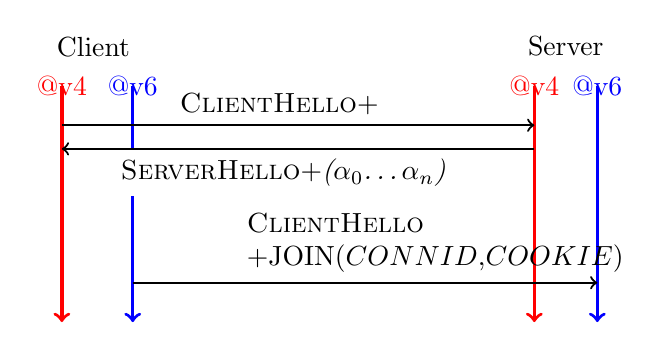
\begin{tikzpicture}
    \colorlet{lightgray}{black!20}
    \tikzstyle{arrow} = [thick,->,>=stealth]
    \tikzset{state/.style={rectangle, dashed, draw, fill=white} }
    \node[black, fill=white] at (0,10) {Client};
    \node[black, fill=white] at (6,10) {Server};
    \node[red, fill=white] at (5.6,9.5) {@v4};
    \node[blue, fill=white] at (6.4,9.5) {@v6};
    \node[red, fill=white] at (-0.4,9.5) {@v4};
    \node[blue, fill=white] at (0.5,9.5) {@v6};
    \draw[red, very thick,->] (-0.4,9.5) -- (-0.4,6.5);
    \draw[blue, very thick,->] (0.5,9.5) -- (0.5,6.5);
    \draw[red, very thick,->] (5.6,9.5) -- (5.6,6.5);
    \draw[blue, very thick,->] (6.4,9.5) -- (6.4,6.5);
   \draw[black, thick, ->] (-0.4,9) -- (5.6,9) node [midway, fill=white, above,
   text width=3cm] {\textsc{ClientHello}+\emph{\tcpls}};
   \draw[black, thick, <-] (-0.4,8.7) -- (5.6,8.7) node [midway, fill=white, below, text width=4.5cm] {\textsc{ServerHello}+\emph{\tcpls($\alpha_0$\ldots$\alpha_n$)} };
   \draw[black, thick, ->] (0.5,7) -- (6.4,7) node [midway, fill=white, above,
   text width=3cm] {\textsc{ClientHello}\\+JOIN($CONNID$,$COOKIE$)};
  \end{tikzpicture}
  \caption{\tcpls supports the attachment of additional \tcp
    connections to a \tcpls connection. Each $\alpha_i$ is encrypted with the
    handshake key.}
  \label{fig:join-example}
\end{figure}
\paragraph*{How to Join}

\tcpls securely solves this \texttt{``connection join''} problem. For example,
consider a client connecting to a dual-stack server. Fig.~\ref{fig:join-example}
depicts the \tls messages exchanged.  The client starts with a
\textsc{ClientHello}. This includes the \tcpls extension to negotiate \tcpls.
The server replies with a \textsc{ServerHello} containing several important and
encrypted control information $\alpha$. First, the server announces its IPv4 and
IPv6 addresses. Second, it associates one connection identifier.  This
identifier uniquely identifies the connection on the server. Third, the server
provides a list of cookies that enable the client to attach additional \tcp
connections to the \tcpls connection. To attach a new connection, e.g., using
the server's IPv6 address, the client opens a \tcp connection and sends a
\textsc{ClientHello} message containing the connection identifier ($CONNID$) and
one of the cookies supplied ($COOKIE$) by the server.

The Connection identifier allows the server to attach the new \tcp connection to
the right \tcpls session, assuming the received cookie is valid. The Connection
identifier and the cookie play that same role as \mptcp's token. However, the
cookie is longer, encrypted in the initial \textsc{ServerHello} message, and
one-time use (i.e., when the server receives a valid cookie, it accepts the
connection, attaches it to the right \tcpls session, and discard the cookie).
Thanks to the cookies, the server can limit the number of \tcp connections that
a client can attach to a \tcpls connection. This prevents some denial-of-service
attacks that are possible with \mptcp.

\subsection{Secure Connection Closing}



%\fr{JOIN is explained here =)}
%Figure~\ref{fig:connmigr} shows a closer look to the \tcpls handshake, and to a
%mpjoin handshake. If the server supports \tcpls, it announces its \tcpLS Encrypted
%Extensions containing the \tcpls connection id \texttt{CONNID}, the list of
%available v4 and v6 addresses from which the sever may be reached, a list of
%one-time use cookies for mpjoin handshakes and lightweight \tcp options. A mpjoin
%handshake is carried out by calling again the \texttt{tcpls\_handshake()} with
%configured handshake properties. This handshake produces a ClientHello with a
%\texttt{JOIN} extension containing information such as the RTT of this
%connection, the \texttt{CONNID} to let the server knows to which \texttt{\tcpls}
%connection bind this \tcp connection, and a \texttt{COOKIE} which acts as an
%authentication mechanism. Note that on-path attackers cannot replay cookies,
%as they are one-time use. However, they can drop the legitimate \texttt{JOIN}
%ClientHello and send the cookie to join the \tcpls's context. The server will
%never send data through a path that has not been confirmed. Confirmation happens
%with a path challenge similar to QUIC, which an on-path attacker in not
%able to answer.

%%\begin{figure}
  %%\begin{tikzpicture}
    %%\colorlet{lightgray}{black!20}
    %%\tikzstyle{arrow} = [thick,->,>=stealth]
    %%\tikzset{state/.style={rectangle, dashed, draw, fill=white} }
    %%\node[black, fill=white] at (0.5,10) {Sender};
    %%\node[black, fill=white] at (6,10) {Receiver};
    %%\node[red, fill=white] at (5.6,9.5) {@v4};
    %%\node[blue, fill=white] at (6.4,9.5) {@v6};
    %%\draw[very thick,->] (0.5,9.5) -- (0.5,0.7);
    %%\draw[red, very thick,->] (5.6,9.5) -- (5.6,0.7);
    %%\draw[blue, very thick,->] (6.4,9.5) -- (6.4,0.7);
    %\node[fill=white] at (0,9) {tcpls\_handshake()};
    %\node[fill=white] at (6,9) {tcpls\_handshake()};
   %\draw[black, thick, ->] (0.5,8) -- (5.6,8) node [midway, fill=white, above,
   %text width=3cm]
   %{Client Hello\\+ extension \tcpls};
   %\draw[black, thick, <-] (0.5,7.7) -- (5.6,7.7) node [midway, fill=white, below,
   %text width=4.5cm] { Server Hello + extension
     %\tcpls+\{CONNID\} + \{ADD\_ADDRS\} + \{COOKIES\} + \{\tcp options\}};
   %\node[fill=white, text width=3cm] at (0.5, 5.5) {Let's migrate on the received
     %v6 addr};
   %\node[fill=white, text width=3cm] at (0.5, 4.5) {tcpls\_handshake()};
   %\draw[black, thick, ->] (0.5,4) -- (6.4,4) node [midway, fill=white, above,
   %text width=3cm]
   %{Client Hello\\+JOIN(CONNID, COOKIE)};
   %\node[fill=white, align=right] at (6.8, 4)
   %{accept()};
   %\node[fill=white, align=right] at (6.1, 3.2)
   %{tcpls\_new()\\tcpls\_handshake()\\tcpls\_accept()};
   %\node[fill=white] at (6.1, 1.9) (Callback) {CB mpjoin!};
   %\node at (7.1, 1.7) (here) {};
   %\draw [->] (Callback) to[out=-80, in=-90,looseness=1.3] (here)
   %to[out=90,in=80,looseness=1.5] (Callback);
   %\node[align=right,fill=white] at (0, 2.5)
   %{tcpls\_stream\_new()\\tcpls\_streams\_attach()\\tcpls\_stream\_close(v4)\\tcpls\_send(v6)};
   %\draw[black, thick, ->] (0.5, 1.2) -- (6.4, 1.2) node [midway, above, text
   %width=3cm] {\{APPDATA\}...\{\tcpls DATA\}...\{APPDATA\}};
  %\end{tikzpicture}
  %\caption{Messages exchanged during an application-level connection migration
    %using \tcpls's API}
  %\label{fig:connmigr}
%\end{figure}


%\begin{figure}
  %\begin{tikzpicture}
    %\colorlet{lightgray}{black!20}
    %\tikzstyle{arrow} = [thick,->,>=stealth]
    %\tikzset{state/.style={rectangle, dashed, draw, fill=white} }
    %\node[black, fill=white] at (0.5,10) {Client};
    %\node[black, fill=white] at (6,10) {Server};
    %\node[red, fill=white] at (5.6,9.5) {@v4};
    %\node[blue, fill=white] at (6.4,9.5) {@v6};
    %\draw[very thick,->] (0.5,9.5) -- (0.5,-2);
    %\draw[red,very thick,->] (6,9.5) -- (6,-2);
    %\draw[blue,very thick,->] (6.2,9.5) -- (6.2,-2);
%%    \node[fill=white] at (0,9) {tcpls\_handshake()};
%%    \node[fill=white] at (6,9) {tcpls\_handshake()};
   %\draw[black, thick, ->] (0.5,8) -- (6,7.5) node [midway, fill=white, above, text width=4cm]
   %{\begin{tabular}{l}SYN\\ClientHello[\tcpls]\end{tabular}};
   %\draw[black, thick, <-] (0.5,7) -- (6,7.5) node [midway, fill=white, below, text width=6cm] {\begin{tabular}{l}SYN+ACK ServerHello[\tcpls(id=123,\\ADDRS(@v4,@v6),C=abc,\ldots)]\end{tabular}};
%%   \node[fill=white, text width=3cm] at (0.5, 4) {Let's migrate on the received
%%     v6 addr};
%%   \node[fill=white, text width=3cm] at (0.5, 3) {tcpls\_handshake()};
   %\draw[black, thick, ->] (0.5,2.5) -- (6.2,2) node [midway, fill=white, above, text width=4cm]
   %{\begin{tabular}{l}SYN,\\ClientHello[JOIN(id=123,C=abc)]\end{tabular}};
%%   \node[fill=white, align=right] at (6.8, 2.5)
%%   {accept()};
%%   \node[fill=white, align=right] at (6.1, 1.7)
%%   {tcpls\_new()\\tcpls\_handshake():};
%%   \node[fill=white] at (6.1, 0.8) (Callback) {CB mpjoin!};
%%   \node at (7.1, 0.6) (here) {};
%%   \draw [->] (Callback) to[out=-80, in=-90,looseness=1.3] (here)
%%   to[out=90,in=80,looseness=1.5] (Callback);
%   \node[fill=white] at (0, 1) {tcpls\_send(on\_v6addr);};
%   \draw[black, thick, ->] (0.5, 0) -- (6, 0) node [midway, above, text
%   width=3cm] {\{APPDATA\}...\{\tcpls DATA\}...\{APPDATA\}};
  %\end{tikzpicture}
%\end{figure}


%-----------------------
\section{TCPLS Prototype}\label{sec:prototype}
%------------------------

\label{sec:content}

This section describes several of the possible benefits of \tcpls
compared to keeping \tcp and \tls isolated.
We provide some use cases and experiment with the
connection application-level connection migration offered by our API. Other user
cases described in Section~\ref{sec:research} are flagged to the roadmap and we
expect them to further demonstrate the
strength of a more intertwined \tls/\tcp transport protocol.

Our current implementation offers: 
%\begin{enumerate}[label=(\roman*)]
\textit{(i)} An experimental API that wraps \tls and \tcp and enables
    applications to 
    handle multihoming, multipathing, and various transport layer mechanisms.
  \textit{(ii)} An improved \tcp extensibility mechanism that sends \tcp options
    through the secure \tcpls channel. We currently support the \tcp
    User Timeout option. Supporting another \tcp option is only a matter of
    extending the sender's API and processing the option
    on the receiver side. \tcpls's internal machinery can already send any \tcp
    option during or after the handshake.
\textit{(iii)} The ability for the server to send eBPF bytecode over the secure
  channel to upgrade the client's \tcp congestion control scheme or
  tune other \tcp mechanisms \cite{brakmo2017tcp, tran2019beyond}.
  \textit{(iv)} The support of parallel streams and multiplexing over \tcp connections
    with different cryptographic context.
%\end{enumerate}

%Note, those features are not stable yet, and many bugs remain to be fixed.

\subsection{More Space for \tcp Options}
\label{sec:tcpoptions}

The \tcp specification limits the size of the entire \tcp header (including options)
to 64 bytes. Unfortunately, the \tcp designers did not foresee that so many \tcp
extensions would be standardized. Today, the size of the \tcp header
becomes a constraint. For example, it severely limits the number of gaps that
can be covered by selective acknowledgments. This gets worse with extensions
such as Multipath \tcp \cite{rfc6824} that consume more space in the \tcp header.
The IETF has discussed this problem for several years, but the latest attempt
to solve it \cite{draft-ietf-tcpm-tcp-edo-10} has not yet been implemented by
major \tcp stacks.

\tcpls provides more space for some \tcp options. First, with \tcpls, \tcp
options can be negotiated during the \tls handshake. Since the \tls messages are
included in the \tcp payload, there is more space to carry them. Another
advantage of this approach is that the TCP options are secured by \tls. This
implies that they cannot be modified by middleboxes. This could be an advantage,
but could also prevent \tcpls from correctly working through some types of
transparent TCP proxies.

Second, we can also carry \tcp options inside \tls records. For example, we used
this feature to implement the \tcp User Time Out option \cite{rfc5482}. A client
can use this option to set the maximum value of the retransmission
timer on a server. Linux \tcp has a socket option that allows setting
this timer locally, but it does not implement the option. With \tcpls, the client sends the option inside a \tls record, the server extracts it
and performs the required \texttt{setsockopt}. 


\subsection{Application-level Connection Migration}
\label{sec:connmigr}

Given the availability of multiple IP paths, connection migration might be a
powerful tool to improve the application connection's reliability.  We
implement Connection migration and Failover as two distinct measures to handle
two different inquiries: 1) The application expects to take advantage of multiple
IP paths. 2) The application expects to be resilient to a network outage. In the
first case, we implement connection migration and multipathing from a
protocol viewpoint, as the same exchange of messages and API calls from \tcpls.
It is left for the application to decide and program
through the API calls whether it wants to move all the traffic from one path to
another or split the traffic among the available paths according. The second
inquiry focuses on simply configuring \tcpls to automatically move the traffic to
another available IP-level path if a network outage is detected. 
%The current implementation supports surviving abrupt reset of the connection,
%yet we may also want to
%monitor the connection and switch to another one if the path quality is low.

Figure~\ref{fig:conn_migration} shows the result of an Application-level
connection migration demo using the API (i.e., it is left to the
application to decide when to migrate, and we expose a simplistic code flow to
perform it). In this experiment, we use an IPMininet network~\cite{ipmininet, jadin2020educational}
composed of a client and a server with a dual-stack of IPs. One path within the
network is composed of OSPF routers with IPv4 only, and one path is composed of
OSPF6 routers IPv6 only. We configure the bandwidth to 30Mbps, the lowest delay
to the v4 link. Our application
downloads a 60 MB file from a server and migrates to the v6 connection in
the middle of the download.

Triggering the connection migration involves chaining 5 API calls:
first, \texttt{tcpls\_handshake()} configured with handshake properties announcing a
JOIN over the v6 connection id. Then, the creation of a new stream
\texttt{tcpls\_stream\_new()} for the v6 connection id, finally followed by the attachment of this new
stream \texttt{tcpls\_streams\_attach()} and the secure closing of the v4 \tcp
connection using \texttt{tcpls\_stream\_close()}. Following these events, the
server seamlessly switches the path while looping over \texttt{tcpls\_send} to
send the file content. Note that all the events trigger callbacks on the server side, to
let the server react appropriately if other requirements need to be fulfilled.

\tcpls's application connection migration takes advantage of multipath to offer
a smooth handover to applications, which QUIC cannot do at the moment.

\begin{figure}
  \centering
  \includegraphics[scale=0.5]{figures/migration.png}
  \caption{Application-level connection migration during a 60MB file download}
  \label{fig:conn_migration}
\end{figure}


%-----------------------------------
\section{Research Agenda}\label{sec:research}
%-----------------------------------

\label{sec:research}
By closely integrating \tcp and \tls, \tcpls opens new research questions
in the transport layer and above. We highlight some of these in this section.

\subsection{A More Secure Multipath TCP}

Multipath TCP \cite{rfc6824, rfc8684} is a recent TCP extension that allows a connection
to send data over different paths. It defines several \tcp options, including
\texttt{ADD\_ADDR} to advertise addresses and \texttt{RM\_ADDR} to remove addresses. Thanks to the \texttt{ADD\_ADDR} option, a dual-stack server can advertise
its IPv6 address over an IPv4 connection initiated by the client. The client can
then use this address to create an IPv6 subflow that is part of the same
connection.

One of the major deployments of Multipath TCP is on Apple's iPhones
\cite{bonaventure2016multipath}. This implementation has decided not to
support the \texttt{ADD\_ADDR} option for security reasons. Since the
Multipath TCP options are sent in clear, an attacker or
a malicious middlebox could try to hijack connections. 
%The latest version
%of Multipath \tcp \cite{rfc8684} addresses this problem by including a
%HMAC in the new \texttt{ADD\_ADDR} option. However, this HMAC uses the key
%that is exchanged in clear during the connection handshake. 
With \tcpls, this
security concern can be addressed elegantly. First, Multipath \tcpls
would not need to exchange a key in clear. It uses cookies (random 128-bits
bitstrings) sent as Encrypted Extensions in the ServerHello during the
handshake, and utilized in \tcpls \texttt{JOIN} handshakes.
Second, in the case of Multipath TCP, the \texttt{ADD\_ADDR} and
\texttt{RM\_ADDR} option could be sent inside \tls records that are encrypted and
authenticated. The information would then reach MP\tcp using a new
\texttt{setsockopt}. Furthermore, since the \tls records are part of the bytestream,
they are reliably delivered in contrast with the new \texttt{ADD\_ADDR} option
that is transmitted unreliably, like all \tcp options, and thus needs to be
echoed.

\subsection{A More Secure \tcp Fast Open}

\tcp Fast Open (TFO) \cite{rfc7413,radhakrishnan2011tcp} is another recent
\tcp extension that allows sending data inside the SYN. TFO defines a
\tcp option that encodes a cookie. This cookie is used to prevent attacks
from spoofed IP addresses. When a client connects first to a server, it sends
an empty cookie but no data in the SYN packet. The server computes a cookie
bound (e.g. using a hash) to the client's IP address and returns it
in the SYN+ACK. For subsequent connections, the client sends its cookie in the SYN
and places data in the payload. The server validates the cookie and processes
the data since it comes from a legitimate IP address. However, the \tcp header
length limits the size of the TFO cookie. \tcpls could easily include
a longer cookie inside the \tls ClientHello within the SYN
payload. This solution would reduce the number of options in the \tcp header
and provide stronger protections against attackers. With this change, \tcpls
would support a 0-RTT connection establishment similar to QUIC. In datacenters and controlled environments, this would work well. However, measurements
are required before deploying that approach in enterprise and
wireless networks as some of them contain middleboxes that block \tcp Fast Open
\cite{paasch2016network}. This middlebox interference has also affected QUIC \cite{langley2017quic} and is thus not specific to \tcp.


\subsection{Pluginizing \tcpls}

PQUIC~\cite{de2019pluginizing} proposed an elegant approach to deploy
QUIC extensions. Instead of waiting for new client and server implementations,
PQUIC includes an eBPF virtual machine to implement new features as bytecode
that can be exchanged over the QUIC connection.
%\tcpls could also be ``pluginized'' like Pluginized QUIC~\cite{de2019pluginizing}. In a nutshell, Plugizined QUIC is a QUIC implementation that includes an eBPF virtual machine and is structured to accept extensions in eBPF bytecode.
%This bytecode that implemnents new protocol features can be loaded from
%disk or exchanged using one the streams of an existing QUIC connection. This
%enables a QUIC server to dynamically push protocol extensions to its clients.

A \tcpls implementation could also be pluginized. The Linux kernel
already includes an eBPF virtual machine~\cite{ebpf:2014}.
It has already been used to develop several types of
\tcp extensions \cite{brakmo2017tcp, tran2019beyond, tran2020beyond}
and recent versions of the mainline kernel allow loading congestion control schemes implemented in eBPF bytecode. \tcpls can transport eBPF bytecode using
\tls records as a second non-data stream.
An interesting research question would be to evaluate the
limits of such a dynamic extensibility? A first intuition to make \tcp's
extensibility mechanism independent from the \tcpls version would be to let \tcpls
communicating plugins to handle new \tcp options and control behaviours, such that the
supported \tcp extensibility capability is not frozen by a given \tcpls
version, but rather dependent on the set of plugins exchanged.

\subsection{Limits to Cross-Layer Integration}

QUIC and \tcpls show that there are benefits in integrating protocols at
adjacent layers. QUIC already integrates HTTP/3~\cite{draft-ietf-quic-http},
but will likely be used by other
applications~\cite{draft-ietf-dprive-dnsoquic,ssh-quic}
in the future. \tcp and \tls are already used by a wide range of
applications~\cite{anderson2019tls}. Should \tcpls also be tuned
for specific applications such as HTTP/3? What are the critical differences
between QUIC and \tcpls from a functionality viewpoint?

%Finally, we would expect to critisize QUIC in light of our \texttt{\tcpls}
%design. We will compare both QUIC and \tcpls, discuss the differences, and analyze
%and answer questions regarding the requirements in transport protocol for today's
%Internet applications.



%\subsection{Plugizing \tcpls}


%Tran shown that the Linux \tcp implementation
%could also be extended using eBPF~\cite{tran2019beyond}. In addition to the
%socketA recent paper 


%This could be added to our prototype, but a more interesting
%research question would be to define a generic API that any \tcpls
%implementation would implement and expose to eBPF

\subsection{Middlebox Interference}

As explained earlier, the deployment of recent \tcp extensions has been
hindered by various types of
middleboxes~\cite{detal2013revealing,medina2004measuring,hesmans2013tcp,edeline2017first}. 
QUIC already suffered from such problems~\cite{langley2017quic}
and many implementations fall back to \tls over \tcp when blocked by a firewall.
Researchers and application developers could include middlebox detection
techniques inside \tcpls. Consider a \tcpls client that copies its \syn header
within a \tcpls message alongside the early data, or makes it part of the
zero-rtt resumption ticket message. By comparing the received \tcp header with
the original one, the server would immediately and reliably detect the presence
of NAT, transparent proxies or other types of middleboxes.  It could then inform
the client and adjust the configuration of their stacks accordingly or fall back
to regular \tcp to preserve connectivity. If deployed, such a protocol would
enable researchers to understand the impact of middleboxes more accurately.

\subsection{Efficient \tcpls Implementations}

During the last years, researchers have proposed
to move transport protocol implementations to user-space
\cite{jeong2014mtcp,marinos2014network} to
kernel bypass techniques such as netmap \cite{rizzo2012revisiting} or
DPDK. In parallel, parts of \tls moved to the Linux kernel
\cite{borkmanncombining} for performance reasons. 
With new results on SmartNICs \cite{firestone2018azure}, it would be
interesting to analyze the best architecture for new \tcpls implementations.
Given the enormous efforts on implementing QUIC\cite{quicimplem},
it would be exciting
to compare QUIC and \tcpls from a performance viewpoint. From a protocol
standpoint, performance advantages of combining those two layers may be
achieved from, for example, adjusting the size of \tls records based on the
current \tcp congestion
window to avoid fragmented records (non-fragmented records makes \tcpls'
design having a zero-copy code path). More generally, we expect many performance
benefits from a more intertwined \tls/\tcp transport protocol at the
cost of design complexity.



%\subsection{What are the Limits of Cross-Layers Integration ?}

%QUIC is a recent example of an integrated protocol since it combines
%transport functions with \tls and application layer functions (HTTP/3). This
%integration can improve performance, but what are its drawbacks ? 


%\newpage

%We expect to investigate several research questions with \tcpls. First, we are
%interested in analyzing how far we can go into supporting \tcp's extensibility
%through our mechanism. Several of new \tcp features may require to inject eBPF
%bytecode to the kernel. It is still unclear how much of \tcp could be extended,
%and if \texttt{\tcpls} may play a role in incentivizing the linux kernel's maintainer
%to support more eBPF in \tcp's implementation, since we now offer a technique to
%propagate eBPF bytecode within authenticated and confidential session with a
%trusted server.

%Second, we expect to analyze several features of \tcpls, such as our
%connection migration, our multipath implementation and our failover mechanism.
%Answering the question about how much \tcpls can or and how fast it performs in
%case of a migration or a network outage.







%\section{Implementation, Deployment \& Research Questions}

%
A \texttt{TCPLS} reference implementation is under active development. The
current implementation is forked from a fast and full
TLS 1.3 implementation written in \texttt{C}. It currently adds about 5k lines
of code (including unit tests and inline code comments) compared to the upstream branch.

The current implementation offers: 
\begin{inparaenum}
  \item An experimental API that wraps TLS and TCP
  \item Our design of TCP's extensibility mechanism throught TCP option sent
within TLS records and processed by TCPLS. We currently support TCP User
Timeout and the injection of eBPF bytecode for TCP's congestion control
algorithm. Supporting another TCP option is only a matter of extending the sender's
API and processing the option
on the receiver side. TCPLS's internal machinery is already implemented for any
type of TCP option to send during the handshake or when the handshake completed.
  \item The support of parallel streams and multiplexing over TCP connections.
    Each stream has its own cryptographic context.
  \item Connection migration and multipathing.
\end{inparaenum}

We expect to investigate several research questions with TCPLS. First, we are
interested in analyzing how far we can go into supporting TCP's extensibility
through our mechanism. Several of new TCP features may require to inject eBPF
bytecode to the kernel. It is still unclear how much of TCP could be extended,
and if \texttt{TCPLS} may play a role in incentivizing the linux kernel's maintainer
to support more eBPF in TCP's implementation, since we now offer a technique to
propagate eBPF bytecode within authenticated and confidential session with a
trusted server.

Second, we expect to analyze several features of TCPLS, such as our
connection migration, our multipath implementation and our failover mechanism.
Answering the question about how much TCPLS can or and how fast it performs in
case of a migration or a network outage.

Finally, we would expect to critisize QUIC in light of our \texttt{TCPLS}
design. We will compare both QUIC and TCPLS, discuss the differences, and analyze
and answer questions regarding the requirements in transport protocol for today's
Internet applications.





%\section{Related Work}

%% !TEX root = ./paper.tex

By closely coupling \tcp and \tls, \tcpls builds upon two of the most important
end-to-end protocols. Given the huge activity on these two protocols within the
research community and the IETF, we restrict our discussion to the closest
related works. Several survey papers provide additional context information
\cite{polese2019survey,li2016multipath,papastergiou2016ossifying}.

Given its security features, \tcpls must be compared with \tcpcrypt
\cite{bittau2010case,rfc8548}. \tcpcrypt predates \tls 1.3. It uses TCP options
to support opportunistic encryption but is not secure against an active network
attacker. \tcpls is compatible with \tls, retains its security properties and supports
additional features. It is also compatible with \tcp middleboxes.

\tcpls also needs to be compared with \mptcp \cite{raiciu2012hard,rfc6824}.
\mptcp supports several coupled congestion control schemes
\cite{peng2014multipath,wischik2011design,khalili2013mptcp} that preserve
fairness even when different paths share the same bottleneck. These are not yet
included in our \tcpls prototype, but could be added with some engineering
effort. The initial idea of coupling \mptcp and \tls was proposed in an expired
Internet draft \cite{draft-paasch-mptcp-ssl-00}, but it was not adopted by the
IETF. MPTCPSec \cite{jadin2017securing} adds security capabilities to \mptcp but
comes with a large performance penalty.

Another important related work is \quic. The initial design
\cite{roskind2013quic} has evolved a lot and large companies have started to
adopt it \cite{langley2017quic,Joras_mvfst,marx2020same}. The \quic
version 1 specification \cite{draft-ietf-quic-transport} supports connection
migration like \tcpls, but we could not test it in our lab since none of the
available open-source implementations have yet implemented it. Multipath
extensions
\cite{viernickel2018multipath,de2017multipath,draft-deconinck-quic-multipath-06,draft-liu-multipath-quic-02}
to \quic have been discussed but not yet adopted within the IETF. Finally, PQUIC
\cite{de2019pluginizing} proposed to carry eBPF code over \quic connections to
deploy new protocol features. This goes beyond the exchange of congestion
control scheme that we demonstrated with \tcpls.

Finally, several solutions have been proposed to provide multipath capabilities
in the application layer. Examples include MP-H2 \cite{nikravesh2019mp} that
extends HTTP/2, MP-DASH \cite{han2016mp} for video streaming or mHTTP
\cite{kim2014multi} that extends HTTP.


\tcpls's idea has also similarities with TLS FOP~\cite{sy2020enhanced}, a
proposal to solve the privacy issue with TFO. However, \tcpls is more generic,
and shows how we can achieve such extensibility work for any other concerns and
new features.

%% Several researchers have proposed techniques to extend various transport
%% protocols. The IETF provides generic guidelines on the design of
%% protocol extensions \cite{rfc6709}. Several researchers have proposed
%% solutions to simplify the implementation of extensions to transport
%% protocols. The closest example include STP \cite{patel2003upgrading}, CTP
%% \cite{bridges2007configurable} and 

%% Patel et al. \cite{patel2003upgrading} propose to use a type-safe version of C to extend a TCP
%% implementation by using bytecode. The implementation of TCPLS completely differs since it uses C to generate eBPF code. Furthemore, by leveraging the
%% flexibility of TLS, TCPLS can securrely exchange various options over a
%% connection. Bridges et al.
%% In CTP, Bridges et al. propose a new protocol that is composed of different microprotocols which can be combined together. In PQUIC, De Coninck et al. \cite{de2019pluginizing} include an eBPF virtual machine inside a QUIC implementation to extend it by using protocol plugins. Our approach is similar from an implementation viewpoint. By combining the TLS and TCP layers, we bring more extensibility to TCP.

%% %maybe
%% % ictcp \cite{wong2001configurable}

%% %configurable and extensible transport \cite{wong2001configurable}

%% % other protocols maybe

%% The IETF has developed various transport protocols, including
%% DCCP \cite{kohler2006designing}, SCTP \cite{rfc4960} and QUIC \cite{draft-ietf-quic-transport}. DCCP brings more flexible congestion control schemes

%% , lots of research but nothing related \cite{nowlan2012fitting}




%% % maybe
%% % Structured streams \cite{ford2007structured}


%% %TCP papers
%% %generic on extensibility

%% %tcp unreliable

%% A wide range of TCP extensions have been proposed \cite{rfc7414}. Some tune
%% protocol implementations with new strategies to retransmit lost data,
%% compute retransmission timers or manage congestion. These do not require
%% the definition of new TCP options that are negotiated during the handshake.
%% Some TCP extensions require the definition of new TCP options. These
%% include the timestamp and large windows extension \cite{rfc7313},
%% the support for selective acknowledgements \cite{rfc2018}, TCP Fast Open
%% \cite{rfc7413} or Multipath TCP \cite{rfc6824}. These extensions are negotiated
%% by exchanging TCP options during the connection handshake. These TCP options
%% allow to extend TCP, but they suffer from several limitations. First,
%% there is limited space in the TCP header to carry them. This limits the
%% number of extensions that can be used for a given TCP connection. The IETF
%% discusses solutions to extend the TCP header space, but the solution is neither
%% finalized nor implemented \cite{draft-ietf-tcpm-tcp-edo-10}. Second, middleboxes
%% interfere with the utilization of new options \cite{honda2011still}. This
%% interference severely limits the extensibility of TCP. TCPLS does not suffer
%% from these problems since the options that it carries are encrypted and can
%% span an entire TLS record (16KBytes).


%% % \cite{nowlan2012fitting}
%% %TODO
%% % idée de combiner des infos de TLS dans MPTCP
%% %\cite{draft-paasch-mptcp-ssl-00}
%% %\cite{jadin2017securing} % secure mptcp


%\section{Discussion}

%\input{discussion}


\section*{Software Artefacts}

A \texttt{TCPLS} reference documentation and implementation is under active development. The
current specifications and code are available on
\url{https://pluginized-protocols.org/tcpls}, forked from a fast and
full TLS 1.3 implementation written in \texttt{C}. Our \tcpls prototype adds
about 5k lines of C code to \texttt{picotls} latest version based on the latest
specification of TLS 1.3.

\section*{Acknowledgments}
We thanks the anonymous reviewers for their helpful feedback, and Mathieu Jadin
for its helpful guidance with IPMininet. This research is supported by the Walloon
Region through the ``Programme de recherche d'interet general
 WALINNOV" - MQUIC project (convention number 1810018).
